\documentclass[letterpaper,11pt]{article}
\oddsidemargin -1.0cm \textwidth 17.5cm

\usepackage[utf8]{inputenc}
\usepackage[activeacute,spanish, es-lcroman]{babel}
\decimalpoint
\usepackage{amsfonts,setspace}
\usepackage{amsmath}
\usepackage{amssymb, amsmath, amsthm}
\usepackage{comment}
\usepackage{float}
\usepackage{amssymb}
\usepackage{dsfont}
\usepackage{anysize}
\usepackage{multicol}
\usepackage{enumerate}
\usepackage{graphicx}
\usepackage[left=1.5cm,top=2cm,right=1.5cm, bottom=1.7cm]{geometry}
\setlength\headheight{1.5em} 
\usepackage{fancyhdr}
\usepackage{multicol}
\usepackage{hyperref}
\usepackage{wrapfig}
\usepackage{subcaption}
\usepackage{siunitx}
\usepackage{cancel}
\usepackage{mdwlist}
\pagestyle{fancy}
\fancyhf{}
\renewcommand{\labelenumi}{\normalsize\bfseries P\arabic{enumi}.}
\renewcommand{\labelenumii}{\normalsize\bfseries (\alph{enumii})}
\renewcommand{\labelenumiii}{\normalsize\bfseries \roman{enumiii})}


\begin{document}

\fancyhead[L]{\itshape{Facultad de Ciencias F\'isicas y Matem\'aticas}}
\fancyhead[R]{\itshape{Universidad de Chile}}

\begin{minipage}{11.5cm}
    \begin{flushleft}
        \hspace*{-0.6cm}\textbf{FI1000-6 Introducción a la Física Clásica}\\
        \hspace*{-0.6cm}\textbf{Profesora:} Claudio Arenas\\
        \hspace*{-0.6cm}\textbf{Auxiliares:} Juan Cristóbal Castro \& Alejandro Bravo\\
        \hspace*{-0.6cm}\textbf{Ayudante:} Mariela Contreras\\
        
    \end{flushleft}
\end{minipage}

\begin{picture}(2,3)
    \put(366, 10){
\includegraphics[scale=0.9]{2020-1/Imágenes/logo/dfi-fcfm.pdf}}
\end{picture}

\begin{center}
	\LARGE\textbf{ Auxiliar \#5 }\\
	\Large{Leyes de Newton}
\end{center}

\vspace{-1cm}
\begin{enumerate}\setlength{\itemsep}{0.4cm}

\rfoot[]{pág. \thepage}

\item[]

\item 2 bloques, de masa $m_1$ y $m_2$, reposan sobre una superficie. En cierto momento una fuerza F se aplica sobre el bloque 2. \\
Estudie el movimiento para los siguientes escenarios:\\
\begin{enumerate}


\item Existe roce entre $m_1$ y $m_2$, pero no entre $m_1$ y el suelo.
\item Existe roce entre $m_1$ y el suelo, pero no entre $m_1$ y $m_2$.
\item No existe roce en el sistema
\item Existe roce tanto entre $m_1$ y $m_2$ como entre $m_1$ y el suelo.
\end{enumerate}

\begin{figure}[h!]
    \centering
    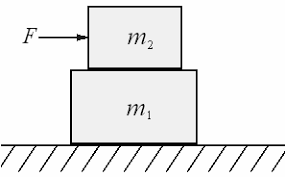
\includegraphics[scale=0.3]{2021-1/Imagenes/ejercicios/images.png}
    \label{fig:my_label}
\end{figure}

\item Demuestre que el problema que se muestra el la figura se puede modelar desde la perspectiva  de una gran masa en movimiento. 
\begin{figure}[h!]
    \centering
    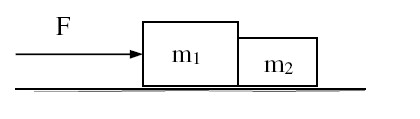
\includegraphics[scale=0.3]{2021-1/Imagenes/ejercicios/images-2.png}
    \label{fig:my_label}
\end{figure}

\item Una bloque de masa m se posa sobre una cuña. Por un lado se conecta con una superficie fija mediante una cuerda ideal. La cuerda es tensada gracias a la acción de la masa colgante M. Por el otro lado, el bloque, se encuentra sujeto a un resorte de constantes k, $l_0$.\\
\begin{figure}[h!]
    \centering
    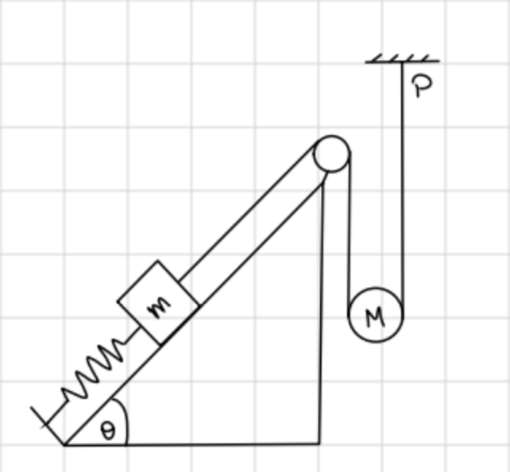
\includegraphics[scale = 0.25]{2020-1/Imágenes/aux8/1.png}
\end{figure}

\begin{enumerate}
    \item Encuentre una razón entre las masas m y M para que el resorte trabaje a tracción y a comprensión. Suponga $\theta$ conocido.
    \item Encuentre $\theta$ tal que el sistema se mantenga en equilibrio
\end{enumerate}

\end{enumerate}
\end{document}